\documentclass{article}

\usepackage{graphicx}
\usepackage{tikz}
\usepackage{tikzsymbols}
\usetikzlibrary{calc,patterns,shapes.geometric}
\pagestyle{empty}
\usepackage[margin=0pt]{geometry}
\geometry{papersize={14in,12in}}

\def\centerarc[#1](#2)(#3:#4:#5){\draw[#1] ($(#2)+({#5*cos(#3)},{#5*sin(#3)})$) arc (#3:#4:#5);}

\begin{document}
	\begin{figure}
		\centering
		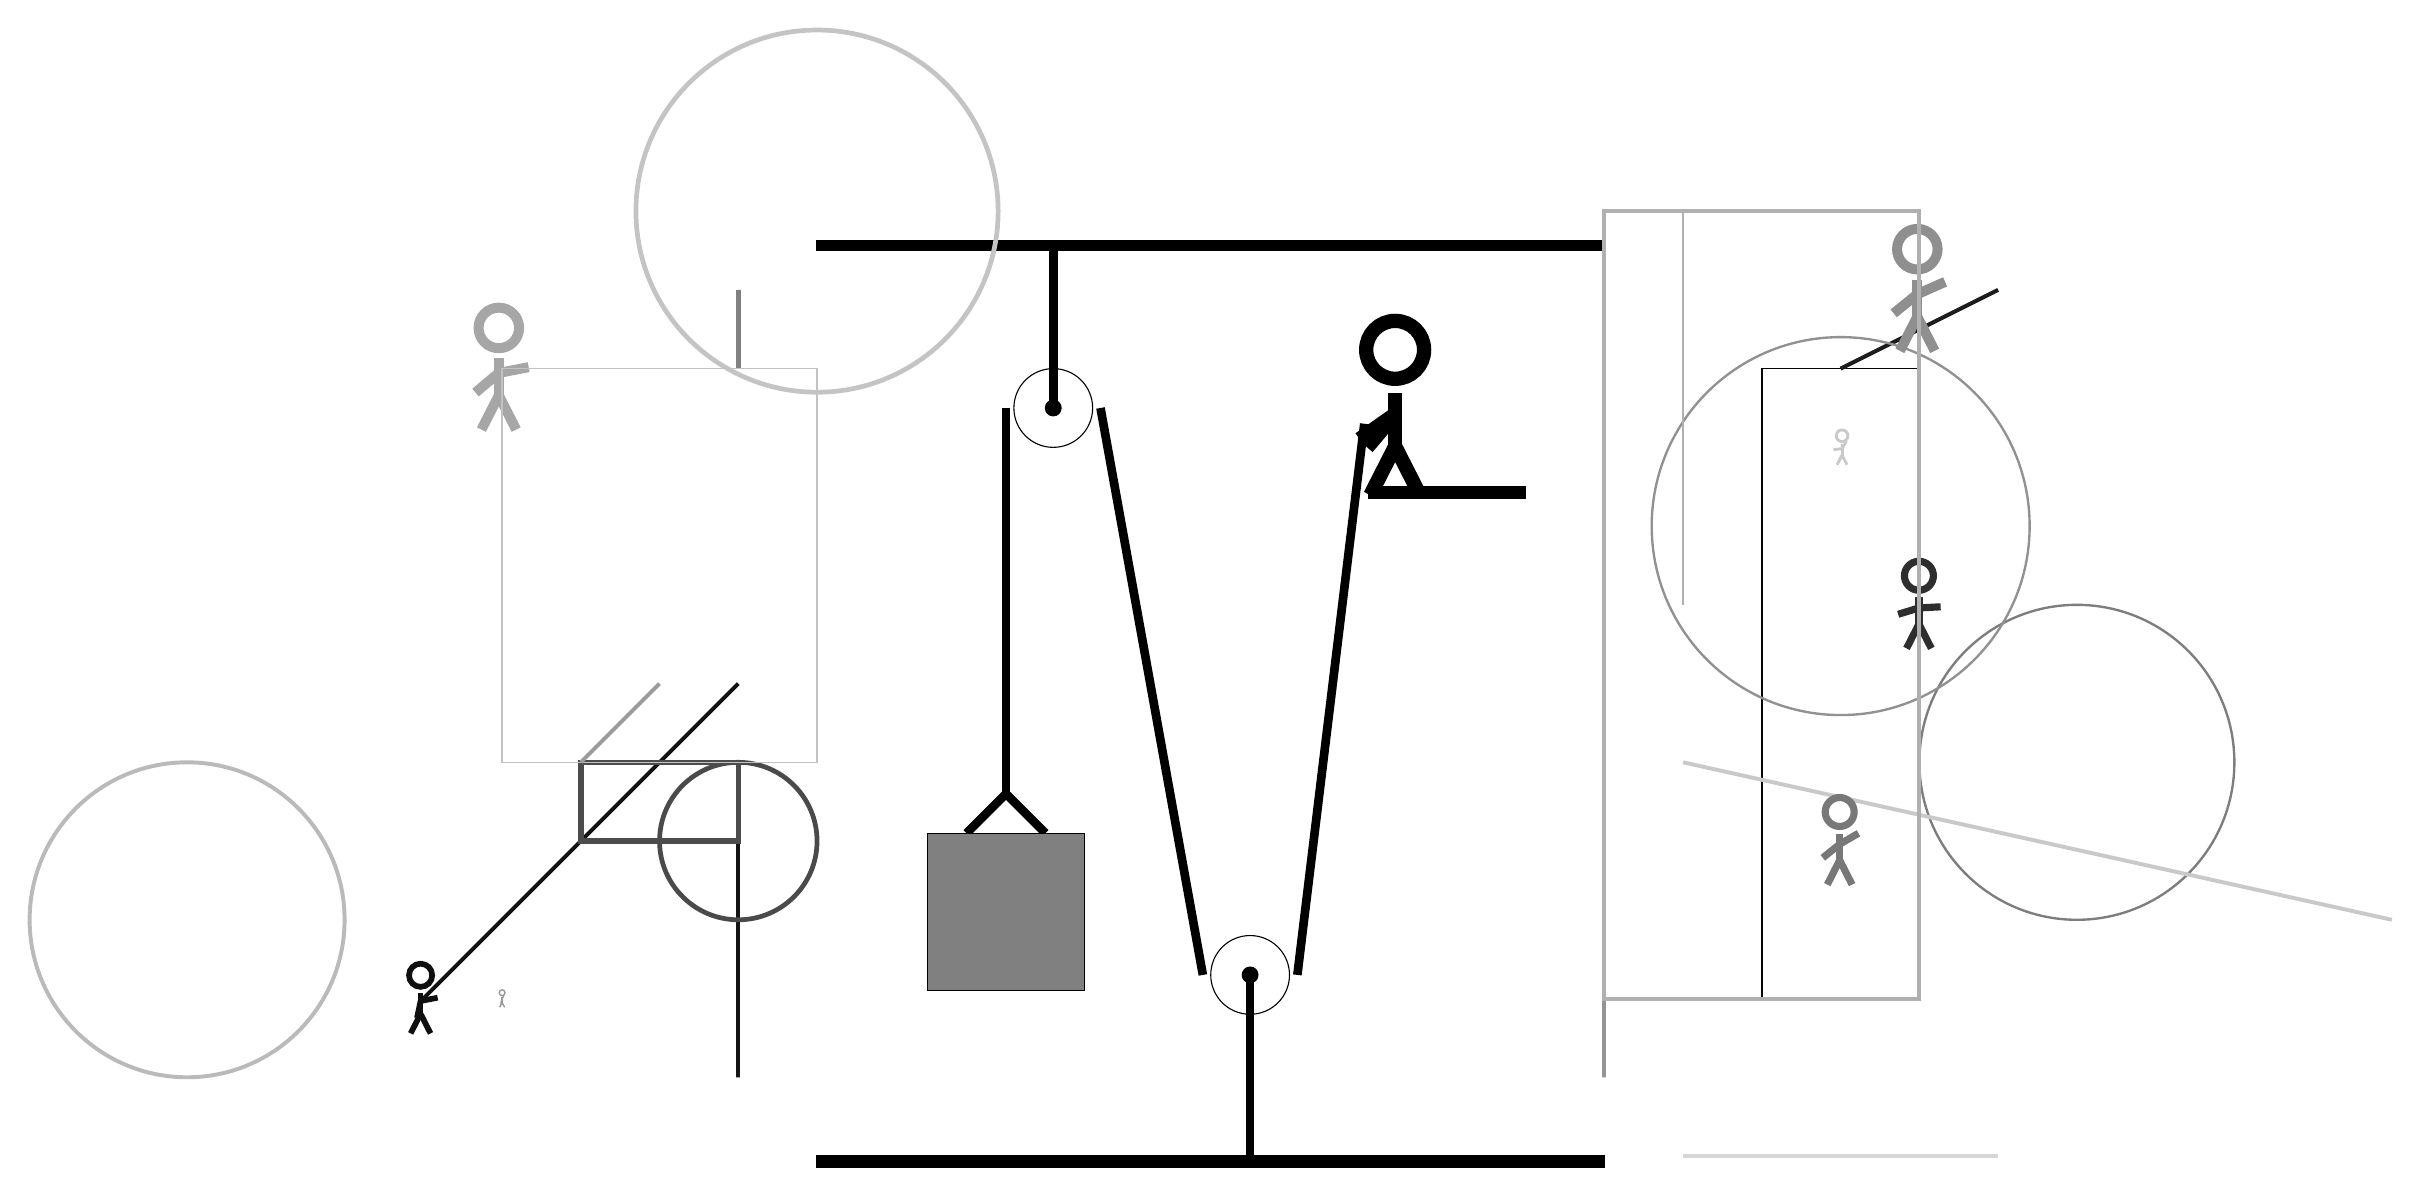
\begin{tikzpicture}
			%%%%% START %%%%%
			
			\draw[fill=black] (-2, 11.5) rectangle (8, 11.625);
			
			\draw (3.5, 2.3) circle (0.5);
			\draw[fill=black] (3.5, 2.3) circle (0.1);
			\draw[line width=1.1mm] (3.5, 2.3) -- (3.5, 0);
			
			\draw (1, 9.5) circle (0.5);
			\draw[fill=black] (1, 9.5) circle (0.1);
			\draw[line width=1.1mm] (1, 11.5) -- (1, 9.5);
			
			\draw[line width=1.1mm](-0.1, 4.1) --  (0.4, 4.6) -- (0.9, 4.1);
			\draw[fill=black!50] (-0.6, 4.1) rectangle (1.4, 2.1);
			
			\draw[line width=1.1mm](0.4, 9.5) -- (0.4, 4.6);
			\centerarc[line width=1.1mm](1, 9.5)(180:0:0.6)
			\draw[line width=1.1mm](1.6, 9.5) -- (2.9, 2.3);
			\centerarc[line width=1.1mm](3.5, 2.3)(180:360:0.6)
			\draw[line width=1.1mm](4.1, 2.3) -- (4.95, 9.3);
			
			\node[line width=0.5mm, color=black!35] at (-6, 10) {\Strichmaxerl[7][40][11]};
			
			\node[line width=0.5mm, color=black!82] at (12, 7) {\Strichmaxerl[5][17][3]};
			\draw[line width=0.5mm, color=black!92] (-3, 5) rectangle (-3, 1);
			\node[line width=0.4mm, color=black!21] at (11, 9) {\Strichmaxerl[2][7][60]};
			\draw[line width=0.5mm, color=black!16](9, 0) -- (13, 0);
			\draw [line width=0.3mm, color=black!51](14, 5) circle (2.0);
			\draw [line width=0.6mm, color=black!71](-3, 4) circle (1.0);
			\draw[line width=0.2mm, color=black!98] (10, 2) rectangle (12, 10);
			\draw[line width=0.5mm, color=black!21](9, 5) -- (18, 3);
			
			\draw[line width=0.5mm, color=black!89](11, 10) -- (13, 11);
			\node[line width=0.2mm, color=black!94] at (-7, 2) {\Strichmaxerl[4][78][11]};
			\node[line width=0.4mm, color=black!53] at (11, 4) {\Strichmaxerl[5][39][30]};
			\draw[line width=0.5mm, color=black!23](11, 12) -- (10, 12);
			\draw[line width=0.5mm, color=black!93](-7, 2) -- (-3, 6);
			\draw[line width=0.6mm, color=black!50] (-3, 10) rectangle (-3, 11);
			\draw [line width=0.3mm, color=black!43](11, 8) circle (2.4);
			
			\node[line width=0.2mm, color=black!40] at (-6, 2) {\Strichmaxerl[1][73][67]};
			\draw[line width=0.2mm, color=black!31] (9, 12) rectangle (9, 7);
			\draw[line width=0.7mm, color=black!70] (-3, 5) rectangle (-5, 4);
			\draw[line width=0.2mm, color=black!24] (-2, 10) rectangle (-6, 5);
			\draw [line width=0.5mm, color=black!27](-10, 3) circle (2.0);
			
			\node[line width=0.3mm, color=black!44] at (12, 11) {\Strichmaxerl[7][39][24]};
			
			\draw[line width=0.5mm, color=black!39](-5, 5) -- (-4, 6);
			\draw [line width=0.6mm, color=black!23](-2, 12) circle (2.3);
			\draw[line width=0.5mm, color=black!42] (8, 9) rectangle (8, 1);
			
			\draw[line width=0.5mm, color=black!31] (8, 2) rectangle (12, 12);
			
			
			\node at (5.3, 9.5) {\Strichmaxerl[10][35][-130]};
			\draw[fill=black] (5, 8.5) rectangle (7, 8.35);
			
			\draw[fill=black] (-2, 0) rectangle (8, -0.15);
			
			%%%%% END %%%%%
		\end{tikzpicture}
	\end{figure}	
\end{document}